\documentclass[a4paper]{article}
\usepackage[a4paper,top=2cm,bottom=2cm,left=1cm,right=1cm,marginparwidth=1.75cm]{geometry}
% \usepackage[spanish]{babel}
% \selectlanguage{spanish}
% \usepackage[utf8]{inputenc}
% \usepackage[T1]{fontenc}
% \usepackage[spanish]{babel}

% \usepackage[T1]{fontenc}
\usepackage{graphicx} %Paquete para usar imagenes
\usepackage{listings}
\usepackage{xcolor}
\usepackage{tcolorbox}

\definecolor{background}{HTML}{E7EBF4}
\definecolor{bg}{HTML}{1a1b26}
\definecolor{fg}{HTML}{a9b1d6}
\definecolor{comment}{HTML}{848cb5}
\definecolor{cyan}{HTML}{82aaff}
\definecolor{orange}{HTML}{ff9e64}
\definecolor{yellow}{HTML}{e9d78e}
\definecolor{purple}{HTML}{c792ea}
\definecolor{green}{HTML}{7fdbca}
\definecolor{numbers}{HTML}{9854f1}
\definecolor{keyword}{HTML}{9854f1}

\lstset{
    showspaces=false, % Evita mostrar espacios en blanco como ␣
    showstringspaces=false,
    inputencoding=utf8,
    extendedchars=true,
    literate=%
    {á}{{\'a}}1
    {é}{{\'e}}1
    {í}{{\'i}}1
    {ó}{{\'o}}1
    {ú}{{\'u}}1
    {ñ}{{\~n}}1
}
\lstdefinestyle{mystyle}{
    language=Python,
    basicstyle=\ttfamily,
    keywordstyle=\color{keyword},
    commentstyle=\color{comment},
    numbers=none,
    numberstyle=\tiny\color{numbers},
    frame=none,
    breaklines=true,
    % showstringspaces=false
    xleftmargin=0mm,
    xrightmargin=0mm,
}

\lstset{style=mystyle}

\newtcolorbox{mycodebox}[1][]{
    arc=7pt,  % Radio de las esquinas redondeadas
    colback=background,  % Color de fondo del cuadro
    boxrule=0.5pt,  % Grosor de la línea del cuadro
    colframe=background,
    width=0.9\textwidth,   % Anchura del cuadro
    % height=5cm,            % Altura del cuadro
    % breakable,
    #1  % Otras opciones personalizadas que puedas necesitar
}


\newtcolorbox{mycodeboxl}[1][]{
    arc=7pt,  % Radio de las esquinas redondeadas
    colback=background,  % Color de fondo del cuadro
    boxrule=0.5pt,  % Grosor de la línea del cuadro
    colframe=background,
    width=0.94\textwidth,   % Anchura del cuadro
    % height=5cm,            % Altura del cuadro
    % breakable,
    #1  % Otras opciones personalizadas que puedas necesitar
}

% Documento
\begin{document}
\newgeometry{left=3cm,right=3cm,top=2cm,bottom=2cm}
\begin{titlepage}

%--------------- Nuevo comendo de linea ----------------->
\newcommand{\linea}{\rule{\linewidth}{0.7mm}} 
\center
%--------------- Universidad, facultad y carrera ----------------->
\textbf{\Large UNIVERSIDAD NACIONAL DE SAN ANTONIO ABAD DEL CUSCO}\\[0.2cm]
\textbf{\Large FACULTAD DE INGENIERÍA ELÉCTRICA, ELECTRÓNICA,INFORMÁTICA Y MECÁNICA}\\[0.2cm]
\textbf{\Large INGENIERÍA INFORMÁTICA Y DE SISTEMAS\\[0.6cm]}

%--------------- Escudos png ----------------->

\includegraphics[width=8cm]{src/escudo-unsaac.png}
\vfill

%--------------- Tema ----------------->
\linea
\\[0.3cm]
% \vfill
\textbf{\LARGE Guía de Laboratorio 3 - Line Clipping}\\[0.2cm]
\linea \\
\vfill

%--------------- Integrantes ----------------->
\textit{\Large Alumno:}\\
%Integrantes del grupo
    \textbf{\large Ian Logan Will Quispe Ventura}\\
    \textit{211359}\\
    % \vfill

%--------------- Profesor y curso ----------------->
\vspace{0.3cm}
    \textit{\Large Docente:}\\
    \textbf{\large Hector Eduardo Ugarte Rojas}\\
\vspace{0.5cm}
    \textit{\Large Curso:}\\
    \textbf{\large Computación Gráfica}\\
    \vfill

\vspace{0.4cm}
    \textbf{\Large Cusco - Perú }\\
    \textbf{\large 2023 - II }\\
    \newpage
    \end{titlepage}

\restoregeometry
\newpage
% •·•·•·•·•·•••·•·•·•·•·•·•·•·•·•·•·•·•·•·•·•·•·•·•·•·•.,..,
% \section{Funcionamiento del algoritmo DDA}
\Large{\textbf{Algoritmo de Cohen-Sutherland en python}}\\[-0.3cm]
\begin{center}
\begin{mycodebox}
\begin{lstlisting}
import sys
from OpenGL.GL import *
from OpenGL.GLU import *
from OpenGL.GLUT import *
 
MAX = 20
TOP, BOTTOM, RIGHT, LEFT = 0x1, 0x2, 0x4, 0x8
ln = [[0] * 4 for _ in range(MAX)]
xmin, ymin, xmax, ymax = 0, 0, 0, 0
lnclip = [[0] * 4 for _ in range(MAX)]
n = 0
k = 0
 
def Plot(ix, iy):
   ix = int(ix)
   iy = int(iy)
   glBegin(GL_POINTS)
   glVertex2i(ix, iy)
   glEnd()
 
def swap(x, y):
   return y, x
 
def dibujaLinea(x0, y0, x1, y1):
   x0 = int(x0)
   y0 = int(y0)
   x1 = int(x1)
   y1 = int(y1)
   dy, x, y, error = 0, 0, 0, 0
   delta_x, delta_y = 0, 0
   steep = abs(y1 - y0) > abs(x1 - x0)
   if steep:
       x0, y0 = swap(x0, y0)
       x1, y1 = swap(x1, y1)
   if x0 > x1:
       x0, x1 = swap(x0, x1)
       y0, y1 = swap(y0, y1)
 
\end{lstlisting}
\end{mycodebox}
\end{center}
\newpage

\begin{center}
\begin{mycodebox}
\begin{lstlisting}
   if y0 > y1:
       dy = -1
   else:
       dy = 1
   delta_x = x1 - x0
   delta_y = abs(y1 - y0)
   y = y0
   error = 0
 
   for x in range(x0, x1 + 1):
       if steep:
           Plot(y, x)
       else:
           Plot(x, y)
       error = error + delta_y
       if 2 * error >= delta_x:
           y = y + dy
           error = error - delta_x
 
def dibujaRectangulo(xmin, ymin, xmax, ymax):
   dibujaLinea(xmin, ymin, xmin, ymax)
   dibujaLinea(xmin, ymax, xmax, ymax)
   dibujaLinea(xmax, ymax, xmax, ymin)
   dibujaLinea(xmax, ymin, xmin, ymin)
 
def calculo_outcode(x, y, xmin, ymin, xmax, ymax):
   oc = 0
   if y > ymax:
       oc |= TOP
   elif y < ymin:
       oc |= BOTTOM
   if x > xmax:
       oc |= RIGHT
   elif x < xmin:
       oc |= LEFT
   return oc
\end{lstlisting}
\end{mycodebox}
\end{center}
\newpage

\begin{center}
\begin{mycodebox}
\begin{lstlisting}
def cohen_sutherland(x0, y0, x1, y1, xmin, ymin, xmax, ymax):
   global k
   in_, done = False, False
   outcode0 = calculo_outcode(x0, y0, xmin, ymin, xmax, ymax)
   outcode1 = calculo_outcode(x1, y1, xmin, ymin, xmax, ymax)
   while not done:
       if (outcode0 | outcode1) == 0:
           done = True
           in_ = True
       elif (outcode0 & outcode1) != 0:
           done = True
       else:
           m = (y1 - y0) / (x1 - x0)
           x, y = 0, 0
           outcode = 0
 
           if outcode0 != 0:
               outcode = outcode0
           else:
               outcode = outcode1
           if (outcode0 & TOP) != 0:
               x = x0 + (ymax - y0) / m
               y = ymax
           elif (outcode & BOTTOM) != 0:
               x = x0 + (ymin - y0) / m
               y = ymin
           elif (outcode & RIGHT) != 0:
               y = y0 + m * (xmax - x0)
               x = xmax
           else:
               y = y0 + m * (xmin - x0)
               x = xmin
           if outcode == outcode0:
               x0, y0 = x, y
               outcode0 = calculo_outcode(x0, y0, xmin, ymin, xmax, ymax)
\end{lstlisting}
\end{mycodebox}
\end{center}

\begin{center}
\begin{mycodebox}
\begin{lstlisting}
           else:
               x1, y1 = x, y
               outcode1 = calculo_outcode(x1, y1, xmin, ymin, xmax, ymax)
 
   print(f"{x0},{y0}---{x1},{y1}")
   if in_:
       lnclip[k][0], lnclip[k][1], lnclip[k][2], lnclip[k][3] = x0, y0, x1, y1
       k += 1
def display2():
   glClear(GL_COLOR_BUFFER_BIT)
   dibujaRectangulo(xmin, ymin, xmax, ymax)
   for i in range(k):
       dibujaLinea(lnclip[i][0], lnclip[i][1], lnclip[i][2], lnclip[i][3])
   glFlush()
 
def display1():
   glClear(GL_COLOR_BUFFER_BIT)
   dibujaRectangulo(xmin, ymin, xmax, ymax)
   for i in range(n):
       dibujaLinea(ln[i][0], ln[i][1], ln[i][2], ln[i][3])
   glFlush()
 
def myinit():
   glClearColor(1.0, 1.0, 1.0, 1.0)
   glColor3f(1.0, 0.0, 0.0)
   glPointSize(1.0)
   glMatrixMode(GL_PROJECTION)
   glLoadIdentity()
   gluOrtho2D(0.0, 499.0, 0.0, 499.0)
\end{lstlisting}
\end{mycodebox}
\end{center}

\begin{center}
\begin{mycodebox}
\begin{lstlisting}
def main():
   global n, xmin, ymin, xmax, ymax
   k = 0
   n = int(input("Ingrese el número de lineas a recortar: "))
   print("Ingrese las coordenadas x - y de los puntos extremos de las lineas:")
   for i in range(n):
       print(f"INGRESE PUNTOS DE LA LINEA {i + 1}:")
       for j in range(4):
           coord_type = "Coordenada X:" if j % 2 == 0 else "Coordenada Y:"
           ln[i][j] = int(input(coord_type))
   print("INGRESE LAS COORDENADAS X-Y DEL RECTANGULO DE RECORTE:")
   xmin = int(input("Ingrese Xmin: "))
   ymin = int(input("Ingrese Ymin: "))
   xmax = int(input("Ingrese Xmax: "))
   ymax = int(input("Ingrese Ymax: "))
   for i in range(n):
       cohen_sutherland(ln[i][0], ln[i][1], ln[i][2], ln[i][3], xmin, ymin, xmax, ymax)
   glutInit(sys.argv)
   glutInitDisplayMode(GLUT_SINGLE | GLUT_RGB)
   glutInitWindowSize(500, 500)
   glutInitWindowPosition(0, 0)
   glutCreateWindow("LINEAS ANTES DEL RECORTE")
   glutDisplayFunc(display1)
   myinit()

   glutInitWindowSize(500, 500)
   glutInitWindowPosition(550, 0)
   glutCreateWindow("LINEAS DESPUES DEL RECORTE")
   glutDisplayFunc(display2)
   myinit()
   glutMainLoop()
if __name__ == "__main__":
   main()
\end{lstlisting}
\end{mycodebox}
\end{center}

Obtención de datos 
\begin{center}
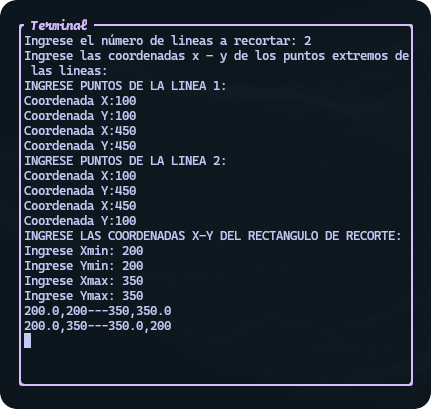
\includegraphics[width=9cm]{src/terminal1.png}
\end{center}


Gráfico generado antes y despues del recorte
\begin{center}
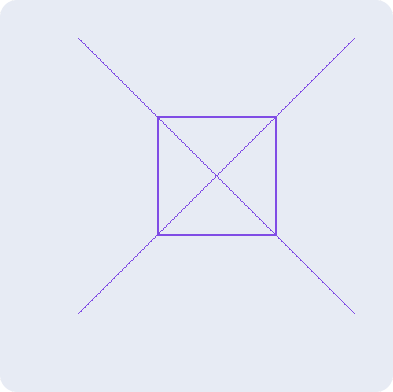
\includegraphics[width=9cm]{src/cohen1.png}

\includegraphics[width=9cm]{src/cohen2.png}
\end{center}
\newpage
% \newpage

\Large{\textbf{Algoritmo paramétrico estudiado en clases}}\\[-0.5cm]
\begin{center}
\begin{mycodebox}
\begin{lstlisting}
import sys
from OpenGL.GL import *
from OpenGL.GLUT import *
from OpenGL.GLU import *
import numpy as np

Xmin, Ymin, Xmax, Ymax = 90, 90, 450,360

def comparacion(x0, y0, x1, y1, Xmin, Ymin, Xmax, Ymax):
    u = 0
    if Xmin <= x0 <= Xmax:
        u = u + 1
    if Ymin <= y0 <= Ymax:
        u = u + 1
    if Xmin <= x1 <= Xmax:
        u = u + 1
    if Ymin <= y1 <= Ymax:
        u = u + 1

    if u == 4:
        line_clipping1(x0, y0, x1, y1, Xmin, Ymin, Xmax, Ymax)
    elif u == 3:
        line_clipping2(x0, y0, x1, y1, Xmin, Ymin, Xmax, Ymax)
    elif u <= 2:
        line_clipping3(x0, y0, x1, y1, Xmin, Ymin, Xmax, Ymax)

def line_clipping1(x0, y0, x1, y1, Xmin, Ymin, Xmax, Ymax):
    dibujaLinea(x0, y0, x1, y1)
\end{lstlisting}
\end{mycodebox}
\end{center}
\newpage

\begin{center}
\begin{mycodeboxl}
\begin{lstlisting}
def line_clipping2(x0, y0, x1, y1, Xmin, Ymin, Xmax, Ymax):
    # Resolviendo el sistema de ecuaciones
    A = np.array([[(x1-x0), -(Xmax - Xmin)], [(y1-y0), -(Ymin - Ymin)]])
    b = np.array([(Xmin-x0), (Ymin-y0)])
    solucion = np.linalg.solve(A, b)
    # Calcular los puntos de corte
    x = x0 + solucion[0] * (x1-x0)
    y = y0 + solucion[0] * (y1-y0)
    dibujaLinea(x0, y0, x, y)

puntos = []
def line_clipping3(x0, y0, x1, y1, Xmin, Ymin, Xmax, Ymax):
    ##########################################
    #    Intersecta con el borde inferior    #
    ##########################################
    # Resolviendo el sistema de ecuaciones
    A = np.array([[(x1-x0), -(Xmax - Xmin)], [(y1-y0), -(Ymin - Ymin)]])
    b = np.array([(Xmin-x0), (Ymin-y0)])
    solucion = np.linalg.solve(A, b)

    # Si se cumple esto entonces la linea intersecta por este borde 
    if 0 <= solucion[0] <= 1:
        X = x0 + solucion[0] * (x1-x0)
        Y = y0 + solucion[0] * (y1-y0)
        puntos.append(X)
        puntos.append(Y)

    ##########################################
    #    Intersecta con el borde superior    #
    ##########################################
    # Resolviendo el sistema de ecuaciones
    A = np.array([[(x1-x0), -(Xmax - Xmin)], [(y1-y0), -(Ymax - Ymax)]])
    b = np.array([(Xmin-x0), (Ymax-y0)])
    solucion = np.linalg.solve(A, b)
\end{lstlisting}
\end{mycodeboxl}
\end{center}
\newpage

\begin{center}
\begin{mycodeboxl}
\begin{lstlisting}
    # Si se cumple esto entonces la linea intersecta por este borde 
    if 0 <= solucion[0] <= 1:
        X = x0 + solucion[0] * (x1-x0)
        Y = y0 + solucion[0] * (y1-y0)
        puntos.append(X)
        puntos.append(Y)

    ###########################################
    #    Intersecta con el borde izquierdo    #
    ########################################### 
    # Resolviendo el sistema de ecuaciones
    A = np.array([[(x1-x0), -(Xmin - Xmin)], [(y1-y0), -(Ymax - Ymin)]])
    b = np.array([(Xmin-x0), (Ymin-y0)])
    solucion = np.linalg.solve(A, b)

    # Si se cumple esto entonces la linea intersecta por este borde 
    if 0 <= solucion[0] <= 1:
        X = x0 + solucion[0] * (x1-x0)
        Y = y0 + solucion[0] * (y1-y0)
        puntos.append(X)
        puntos.append(Y)

    #########################################
    #    Intersecta con el borde derecho    #
    ######################################### 
    # Resolviendo el sistema de ecuaciones
    A = np.array([[(x1-x0), -(Xmax - Xmax)], [(y1-y0), -(Ymax - Ymin)]])
    b = np.array([(Xmax-x0), (Ymin-y0)])
    solucion = np.linalg.solve(A, b)

    # Si se cumple esto entonces la linea intersecta por este borde 
    if 0 <= solucion[0] <= 1:
        X = x0 + solucion[0] * (x1-x0)
        Y = y0 + solucion[0] * (y1-y0)
        puntos.append(X)
        puntos.append(Y)

\end{lstlisting}
\end{mycodeboxl}
\end{center}
\newpage
\begin{center}
\begin{mycodebox}
\begin{lstlisting}
    # Dibujar la linea recortada con los puntos de intersección 
    dibujaLinea(puntos[0], puntos[1], puntos[2], puntos[3])
    glFlush()
# Necesario para dibujar las lineas
def Plot(ix, iy):
   ix = int(ix)
   iy = int(iy)
   glBegin(GL_POINTS)
   glVertex2i(ix, iy)
   glEnd()
def swap(x, y):
   return y, x
# Algortimo de Bresenham
def dibujaLinea(x0, y0, x1, y1):
   x0 = int(x0)
   y0 = int(y0)
   x1 = int(x1)
   y1 = int(y1)
   dy, x, y, error = 0, 0, 0, 0
   delta_x, delta_y = 0, 0
   steep = abs(y1 - y0) > abs(x1 - x0)
   if steep:
       x0, y0 = swap(x0, y0)
       x1, y1 = swap(x1, y1)
   if x0 > x1:
       x0, x1 = swap(x0, x1)
       y0, y1 = swap(y0, y1)
   if y0 > y1:
       dy = -1
   else:
       dy = 1
   delta_x = x1 - x0
   delta_y = abs(y1 - y0)
   y = y0
   error = 0
   for x in range(x0, x1 + 1):
       if steep:
           Plot(y, x)

\end{lstlisting}
\end{mycodebox}
\end{center}
\newpage
\begin{center}
\begin{mycodebox}
\begin{lstlisting}
       else:
           Plot(x, y)
       error = error + delta_y
       if 2 * error >= delta_x:
           y = y + dy
           error = error - delta_x

def dibujaRectangulo(xmin, ymin, xmax, ymax):
   dibujaLinea(xmin, ymin, xmin, ymax)
   dibujaLinea(xmin, ymax, xmax, ymax)
   dibujaLinea(xmax, ymax, xmax, ymin)
   dibujaLinea(xmax, ymin, xmin, ymin)

# Primera venta
def display1():
   glClear(GL_COLOR_BUFFER_BIT)
   glColor3f(0.5, 0.3, 0.9) 
   glPointSize(2.0)
   dibujaRectangulo(Xmin, Ymin, Xmax, Ymax)
   glPointSize(1.0)
   glColor3f(0.8431372549019608, 0.3686274509803922, 1.0)
   dibujaLinea(180, 120, 360, 300)
   dibujaLinea(120, 120, 210, 60)
   dibujaLinea(30, 180, 300, 450)
   glFlush()

def display2():
   glClear(GL_COLOR_BUFFER_BIT)
   glColor3f(0.5, 0.3, 0.9) 
   glPointSize(1.0)
   dibujaRectangulo(Xmin, Ymin, Xmax, Ymax)
   glPointSize(2.0)
   glColor3f(0.8156862745098039, 0.26666666666666666, 1.0)
   comparacion(180, 120, 360, 300, 90, 90, 450,360)
   comparacion(120, 120, 210, 60, 90, 90, 450,360)
   comparacion(30, 180, 300, 450, 90, 90, 450,360)
   glFlush()
\end{lstlisting}
\end{mycodebox}
\end{center}
\newpage
\begin{center}
\begin{mycodebox}
\begin{lstlisting}
def myinit():
   glClearColor(0.9058823529411765, 0.9215686274509803, 0.9568627450980393, 1.0)
   glColor3f(1.0, 0.0, 0.0)
   glPointSize(1.0)
   glMatrixMode(GL_PROJECTION)
   glLoadIdentity()
   gluOrtho2D(0.0, 499.0, 0.0, 499.0)

glutInit(sys.argv)
glutInitDisplayMode(GLUT_SINGLE | GLUT_RGB)
# Primera ventana
glutInitWindowSize(500, 500)
glutInitWindowPosition(0, 0)
glutCreateWindow("Lineas antes del recorte")
glutDisplayFunc(display1)
myinit()

glutInitWindowSize(500, 500)
glutInitWindowPosition(550, 0)
# Segunda ventana
glutCreateWindow("Lineas despues del recorte")
glutDisplayFunc(display2)
myinit()
glutMainLoop()

\end{lstlisting}
\end{mycodebox}
\end{center}
\newpage
Gráfico generado antes y despues del recorte
\begin{center}
    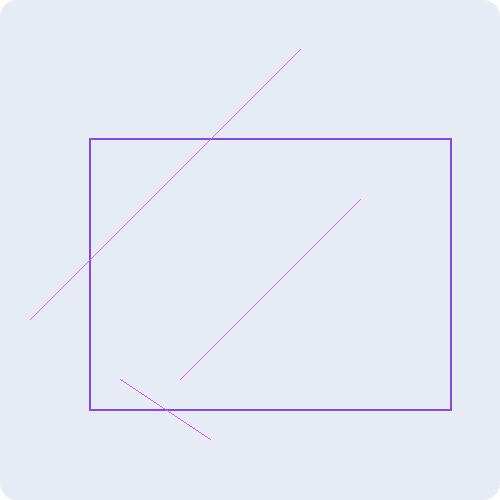
\includegraphics[width=12cm]{src/clipping1.png}\\[0.2cm]
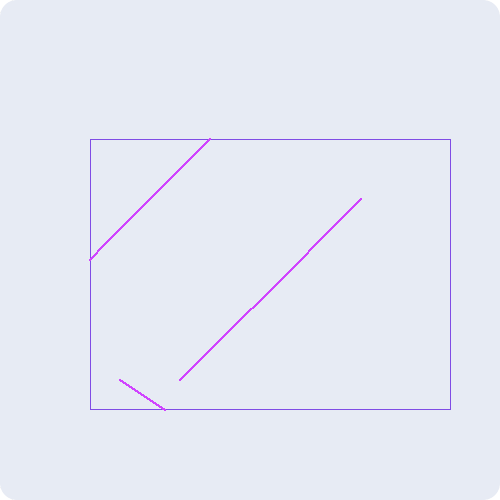
\includegraphics[width=12cm]{src/clipping2.png}
\end{center}
\newpage

\end{document}
